\documentclass[11pt,a4paper]{article}

% IOS Press FAIA style packages
\usepackage[utf8]{inputenc}
\usepackage[T1]{fontenc}
\usepackage{newunicodechar}
\DeclareTextCommandDefault{\h}[1]{#1}
\usepackage{times}
\usepackage{amsmath,amssymb}
\usepackage{graphicx}
\usepackage{booktabs}
\usepackage{multirow}
\usepackage{url}
\usepackage{float}
\usepackage[hidelinks]{hyperref}

% TikZ for diagrams
\usepackage{tikz}
\usetikzlibrary{shapes.geometric, arrows.meta, positioning, fit, backgrounds, calc}

% pgfplots for charts
\usepackage{pgfplots}
\pgfplotsset{compat=1.18}

% checkmark
\usepackage{amssymb}

% Page layout for IOS Press
\usepackage[top=2.3cm,bottom=2.3cm,left=2cm,right=2cm]{geometry}
\setlength{\parindent}{0.5cm}
\setlength{\parskip}{0pt}

% Two-column layout
\usepackage{multicol}
\setlength{\columnsep}{0.5cm}

% Section formatting
\usepackage{titlesec}
\titleformat{\section}{\normalfont\bfseries}{\thesection.}{0.5em}{}
\titleformat{\subsection}{\normalfont\bfseries\itshape}{\thesubsection.}{0.5em}{}
\titleformat{\subsubsection}{\normalfont\itshape}{\thesubsubsection.}{0.5em}{}
\titlespacing*{\section}{0pt}{1.2ex plus 0.5ex minus 0.2ex}{0.8ex plus 0.2ex}
\titlespacing*{\subsection}{0pt}{1.0ex plus 0.3ex minus 0.2ex}{0.5ex plus 0.1ex}
\titlespacing*{\subsubsection}{0pt}{0.8ex plus 0.2ex minus 0.1ex}{0.3ex plus 0.1ex}

% Caption formatting
\usepackage{caption}
\captionsetup{font=small,labelfont=bf,skip=4pt}

% Tighter spacing
\setlength{\textfloatsep}{8pt}
\setlength{\floatsep}{6pt}
\setlength{\intextsep}{6pt}

% Ensure text returns to justified after captionof
\usepackage{ragged2e}

% amsthm for definitions
\usepackage{amsthm}
\newtheorem{definition}{Definition}

\begin{document}

% Title
\begin{center}
{\Large\bfseries A Three-Tier Knowledge Graph RAG\\[0.3em] for Vietnamese Legal Question Answering}\\[1.5em]

{\normalsize
Le Hong Hien$^{a,1}$, Nguyen Dinh Hien$^{a}$, Ngo Quoc Hung$^{b}$ and Dang Viet Dung$^{a}$\\[0.5em]
$^a$\textit{Faculty of Computer Science, University of Information Technology,}\\
\textit{Vietnam National University Ho Chi Minh City, Vietnam}\\
$^b$\textit{School of Computer Science, University College Dublin, Ireland}\\[1em]
}
\end{center}

\noindent\textbf{Abstract.} Answering legal questions accurately requires navigating hierarchical document structures, following cross-references, and performing multi-hop reasoning---capabilities that standard Retrieval Augmented Generation (RAG) systems lack. This gap is especially pronounced in Vietnamese legal text, where tonal language, domain-specific abbreviations, and a rigid structural hierarchy (Law$\to$Chapter$\to$Article$\to$Clause$\to$Point) compound retrieval difficulty. We propose a three-tier knowledge graph RAG architecture that extends the Legal-Onto Rela-model with a formal knowledge model $\mathcal{M} = (\mathcal{O}, \mathcal{G}, \mathcal{T}, \Phi)$, integrating an OWL ontology for terminological knowledge, a domain-specific knowledge graph for assertional knowledge, and a document tree forest for structural navigation. The three retrieval tiers---LLM-guided tree traversal, dual-level semantic retrieval with intent-aware Personalized PageRank, and Reciprocal Rank Fusion---operate over these complementary representations. Experiments on 375 real Vietnamese legal questions show that our system achieves 75.2\% Hit@10 (MRR 0.545), outperforming BM25 (26.7\%), semantic search (15.8\%), LightRAG (33.9\%), and PageIndex (35.2\%) by substantial margins. Ablation studies confirm each tier's additive contribution, with Tier~3 fusion providing 4.0 percentage points over Tier~1+2 alone. To our knowledge, this is the first system to combine ontology-enhanced knowledge graphs with multi-tier retrieval for Vietnamese legal question answering.\\[0.5em]

\noindent\textbf{Keywords.} Knowledge Graph, Legal Question Answering, Retrieval Augmented Generation, Ontology, Vietnamese NLP, Multi-Tier Retrieval

\begin{multicols}{2}

\section{Introduction}

Legal question answering (QA) systems serve a growing need as citizens and businesses seek to understand their rights and obligations. However, building effective systems for this domain presents challenges that distinguish it from general-purpose QA.

Legal documents exhibit \textbf{complex hierarchical structures}. A single law may organize content into parts, chapters, sections, articles, clauses, and points, where each level carries distinct legal scope. Understanding these structural relationships is essential for accurate retrieval: an article on shareholder voting rights only applies within the chapter governing joint-stock companies.

Legal texts also contain pervasive \textbf{cross-references}. An article defining establishment conditions may reference another specifying required documents, which in turn points to procedures defined elsewhere. Answering a practical question like ``Can a foreign investor establish a limited liability company in Vietnam?'' requires following reference chains across multiple articles to assemble conditions, procedures, and exceptions.

The \textbf{Vietnamese legal domain} introduces additional complexity. Vietnamese is a tonal language with compound words whose boundaries are ambiguous without segmentation. Legal practitioners use extensive abbreviations (\textit{H\DJ QT} for ``H\d{o}i d\`{o}ng qu\h{a}n tr\d{i}'', \textit{CTCP} for ``C\^{o}ng ty c\h{o} ph\`{a}n'') that general-purpose models do not recognize. Moreover, Vietnamese law follows a rigid hierarchy---Constitution, Codes, Decrees, Circulars---where document type determines legal authority and interpretation precedence.

Traditional RAG systems \cite{ref2} rely on vector similarity between query and document embeddings \cite{ref_sbert}. While effective for many domains \cite{ref_gao2024,ref_fan2024}, this approach faces three fundamental limitations for legal QA: (1)~a \textbf{semantic gap} where legal terminology has precise meanings that general embeddings miss, (2)~\textbf{no structural awareness} since vector similarity treats documents as flat text, and (3)~\textbf{no reasoning capability} since dense retrieval cannot follow reference chains or apply legal inference.

No existing system addresses all three limitations simultaneously. Graph-based approaches like LightRAG \cite{ref5} and GraphRAG \cite{ref4} model entity relationships but ignore document hierarchy. PageIndex \cite{ref14} navigates hierarchical structure but lacks semantic reasoning. Legal ontology systems \cite{ref6,ref8} represent domain knowledge but are not integrated with modern retrieval architectures. The intersection of ontology-enhanced knowledge graphs, multi-tier retrieval, and Vietnamese legal processing remains unexplored.

We propose a \textbf{three-tier knowledge graph RAG} architecture that addresses these gaps through:
\begin{enumerate}
\item \textbf{LLM-guided tree traversal} through document hierarchies for structural navigation (Tier~1),
\item \textbf{Dual-level semantic retrieval} with intent-aware Personalized PageRank on a domain knowledge graph (Tier~2),
\item \textbf{Reciprocal Rank Fusion} for cross-tier merging with knowledge graph expansion (Tier~3).
\end{enumerate}

Our contributions are as follows. First, we propose a three-tier RAG architecture that combines structural, semantic, and graph-based retrieval. Second, we construct a Vietnamese legal knowledge graph with 1,299 entities across 11 types and 2,577 relations across 30 types, with LLM-based extraction and Vietnamese slug normalization for deduplication. Third, we introduce a multi-intent Personalized PageRank algorithm that adapts edge weights based on detected query intents. Fourth, we conduct comprehensive experiments on 375 real legal questions demonstrating 75.2\% Hit@10 (+41.3pp over the best baseline), with ablation studies confirming each tier's contribution.

The remainder of this paper is organized as follows. Section~\ref{sec:related} reviews related work. Section~\ref{sec:method} describes our methodology. Section~\ref{sec:experiments} presents experiments. Section~\ref{sec:discussion} discusses findings. Section~\ref{sec:conclusion} concludes.

\section{Related Work}
\label{sec:related}

\subsection{Retrieval-Augmented Generation}

Retrieval-Augmented Generation (RAG) \cite{ref2} enhances language models by grounding generation in retrieved evidence. The field has evolved from basic retrieve-then-read pipelines \cite{ref3} to advanced architectures incorporating self-reflection \cite{ref_selfrag}, corrective retrieval \cite{ref_crag}, and hypothetical document generation \cite{ref_hyde}. Comprehensive surveys \cite{ref_gao2024,ref_fan2024} document this progression toward modular and agentic RAG systems. However, most advances target general-domain QA and do not address the structural and semantic requirements of legal text.

\subsection{Knowledge Graphs in Information Retrieval}

Knowledge graph (KG) augmented retrieval has gained traction through systems like GraphRAG \cite{ref4}, which constructs KGs from documents for multi-hop reasoning and global summarization, and LightRAG \cite{ref5}, which provides lightweight entity-relation extraction. KG embedding methods including TransE \cite{ref_transe} and RotatE \cite{ref_rotateE} learn entity representations in multi-relational graphs, while Personalized PageRank \cite{ref12,ref_jeh2003} computes query-specific node importance. PageIndex \cite{ref14} introduced LLM-guided tree traversal for hierarchical navigation using document structure summaries. These approaches address individual aspects---graph reasoning, structural navigation---but none combines them into a unified multi-tier framework.

\subsection{Legal NLP and QA Systems}

Legal information retrieval has progressed from lexical methods \cite{ref1,ref11} to neural approaches using domain-adapted models like LEGAL-BERT \cite{ref_chalkidis}. Ontology-based representations \cite{ref8} formalize legal concepts and relations, with Legal-Onto \cite{ref6} integrating the Rela-model \cite{ref10} with conceptual graphs for Vietnamese Land Law. For Vietnamese NLP, PhoBERT \cite{ref_phobert} and VnCoreNLP \cite{ref_vncorenlp} provide foundational capabilities, while Ngo et al.~\cite{ref7} designed a QA system using BM25, BERT \cite{ref13}, and legal domain knowledge. Broader surveys \cite{ref_zhong2020,ref_legalai2024} document the challenges of applying NLP to legal text, including specialized vocabulary and complex reasoning requirements. However, no existing system combines ontology-enhanced KGs with multi-tier retrieval for Vietnamese legal QA.

\subsection{Positioning}

Table~\ref{tab:related-comparison} compares key features across systems. Our approach is the first to unify knowledge graph reasoning, domain ontology, tree navigation, intent-aware retrieval, and rank fusion in a single architecture.

\vspace{0.3em}
\noindent
\centering\scriptsize
\captionof{table}{Feature comparison of RAG systems.}
\label{tab:related-comparison}
\begin{tabular}{l@{\hskip 4pt}c@{\hskip 4pt}c@{\hskip 4pt}c@{\hskip 4pt}c@{\hskip 4pt}c}
\toprule
\textbf{Feature} & \textbf{BM25} & \textbf{Light} & \textbf{Graph} & \textbf{Page} & \textbf{Ours} \\
\midrule
Knowledge Graph & -- & \checkmark & \checkmark & -- & \checkmark \\
Multi-tier & -- & -- & -- & -- & \checkmark \\
Intent-aware & -- & -- & -- & -- & \checkmark \\
Domain Ontology & -- & -- & -- & -- & \checkmark \\
Tree Navigation & -- & -- & -- & \checkmark & \checkmark \\
Rank Fusion & -- & -- & -- & -- & \checkmark \\
\bottomrule
\end{tabular}
\normalsize
\justifying
\vspace{0.3em}

\section{Methodology}
\label{sec:method}

\subsection{Problem Formulation}

Given a legal corpus $\mathcal{D} = \{d_1, d_2, \ldots, d_m\}$ where each document $d_i$ contains articles $\{a_{i,1}, \ldots, a_{i,n_i}\}$ organized hierarchically, and a natural language query $q$, the task is to retrieve a ranked list of articles $A^* = [a_1^*, a_2^*, \ldots, a_k^*]$ that are relevant to answering $q$.

We construct a knowledge model $\mathcal{M}$ from $\mathcal{D}$ and define retrieval as:
\begin{equation}
A^* = \Phi(q, \mathcal{M}) \quad\text{where}\quad \mathcal{M} = (\mathcal{O}, \mathcal{G}, \mathcal{T}, \Phi)
\end{equation}

The model $\mathcal{M}$ integrates four components: ontology $\mathcal{O}$ for terminological knowledge, knowledge graph $\mathcal{G}$ for assertional knowledge, document forest $\mathcal{T}$ for structural knowledge, and retrieval functions $\Phi$ that operate over these representations.

\subsection{System Overview}

Figure~\ref{fig:architecture} illustrates the architecture. The \textbf{offline phase} constructs $\mathcal{M}$ from legal documents through parsing, entity-relation extraction, and ontology generation. The \textbf{online phase} processes queries through ontology-based expansion (Stage~0) followed by three retrieval tiers that leverage $\mathcal{T}$, $\mathcal{G}$, and $\mathcal{O}$ respectively.

\end{multicols}

% Figure 1: System Architecture
\begin{figure}[H]
\centering
\resizebox{\textwidth}{!}{%
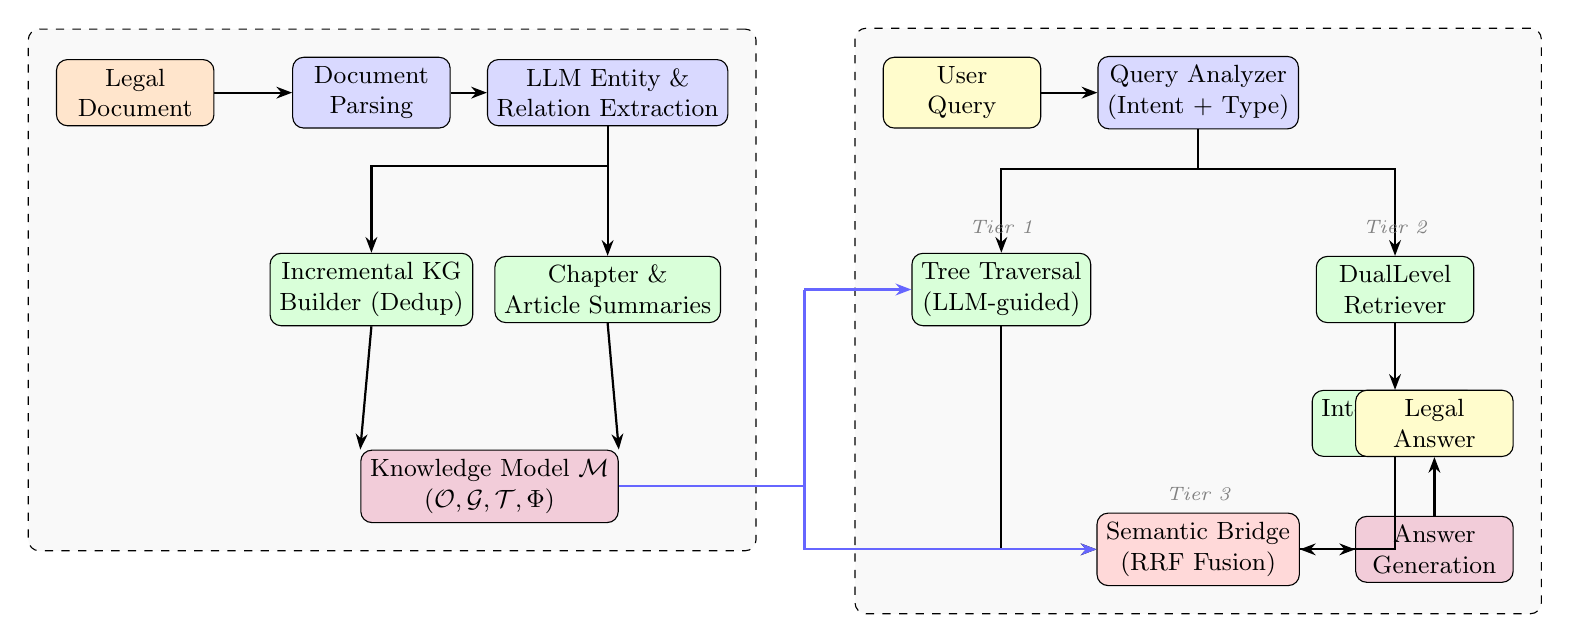
\begin{tikzpicture}[
    % Styles
    box/.style={rectangle, draw, rounded corners, minimum height=0.8cm, minimum width=2cm, align=center, font=\small},
    phase/.style={rectangle, draw, dashed, rounded corners, inner sep=10pt},
    tier/.style={rectangle, draw, dashed, rounded corners, inner sep=8pt, fill=blue!3},
    arrow/.style={-{Stealth[length=2mm]}, thick},
    dataarrow/.style={-{Stealth[length=2mm]}, thick, blue!60},
    label/.style={font=\footnotesize\bfseries},
]

% === OFFLINE PHASE (Left) ===
\node[box, fill=orange!20] (doc) at (0,0) {Legal\\Document};
\node[box, fill=blue!15] (parse) at (3,0) {Document\\Parsing};
\node[box, fill=blue!15] (extract) at (6,0) {LLM Entity \&\\Relation Extraction};
\node[box, fill=green!15] (kgbuild) at (3,-2.5) {Incremental KG\\Builder (Dedup)};
\node[box, fill=green!15] (summary) at (6,-2.5) {Chapter \&\\Article Summaries};
\node[box, fill=purple!20, minimum width=3cm] (kg) at (4.5,-5) {Knowledge Model $\mathcal{M}$\\$(\mathcal{O}, \mathcal{G}, \mathcal{T}, \Phi)$};

% Offline arrows
\draw[arrow] (doc) -- (parse);
\draw[arrow] (parse) -- (extract);
\draw[arrow] (extract.south) -- ++(0,-0.5) -| (kgbuild.north);
\draw[arrow] (extract.south) -- ++(0,-0.5) -| (summary.north);
\draw[arrow] (kgbuild.south) -- (kg.north west);
\draw[arrow] (summary.south) -- (kg.north east);

% Offline phase box
\begin{scope}[on background layer]
\node[phase, fill=gray!5, fit=(doc)(parse)(extract)(kgbuild)(summary)(kg), label={[label]above:Offline Phase: Knowledge Model Construction}] (offline) {};
\end{scope}

% === ONLINE PHASE (Right) ===
\node[box, fill=yellow!20] (query) at (10.5,0) {User\\Query};
\node[box, fill=blue!15] (analyzer) at (13.5,0) {Query Analyzer\\(Intent + Type)};

% Tier 2 (runs first)
\node[box, fill=green!15] (dual) at (16,-2.5) {DualLevel\\Retriever};
\node[box, fill=green!15] (ppr) at (16,-4.2) {Intent-Aware\\PPR};

% Tier 1
\node[box, fill=green!15] (tree) at (11,-2.5) {Tree Traversal\\(LLM-guided)};

% Tier 3
\node[box, fill=red!15] (bridge) at (13.5,-5.8) {Semantic Bridge\\(RRF Fusion)};
\node[box, fill=purple!20] (gen) at (16.5,-5.8) {Answer\\Generation};
\node[box, fill=yellow!20] (answer) at (16.5,-4.2) {Legal\\Answer};

% Online arrows
\draw[arrow] (query) -- (analyzer);
\draw[arrow] (analyzer.south) -- ++(0,-0.5) -| (tree.north);
\draw[arrow] (analyzer.south) -- ++(0,-0.5) -| (dual.north);
\draw[arrow] (dual) -- (ppr);
\draw[arrow] (tree.south) |- (bridge.west);
\draw[arrow] (ppr.south) |- (bridge.east);
\draw[arrow] (bridge) -- (gen);
\draw[arrow] (gen) -- (answer);

% KG to Online connections
\coordinate (splitpt) at (8.5,-5);
\draw[blue!60, thick] (kg.east) -- (splitpt);
\draw[blue!60, thick] (splitpt) -- (8.5,-2.5);
\draw[dataarrow] (8.5,-2.5) -- (tree.west);
\draw[dataarrow] (splitpt) -- (8.5,-5.8) -- (bridge.west);

% Tier labels
\node[font=\scriptsize\itshape, gray] at (11,-1.7) {Tier 1};
\node[font=\scriptsize\itshape, gray] at (16,-1.7) {Tier 2};
\node[font=\scriptsize\itshape, gray] at (13.5,-5.1) {Tier 3};

% Online phase box
\begin{scope}[on background layer]
\node[phase, fill=gray!5, fit=(query)(analyzer)(tree)(dual)(ppr)(bridge)(gen)(answer), label={[label]above:Online Phase: Three-Tier Query Processing}] (online) {};
\end{scope}

\end{tikzpicture}
}
\caption{System architecture. The offline phase constructs knowledge model $\mathcal{M}$ from legal documents. The online phase processes queries through three tiers: dual-level semantic retrieval with PPR (Tier~2, runs first for global coverage), LLM-guided tree traversal (Tier~1), and RRF-based fusion with KG expansion (Tier~3).}
\label{fig:architecture}
\end{figure}

\begin{multicols}{2}

\subsection{Knowledge Representation Model}

Our knowledge model extends the Legal-Onto framework \cite{ref6}, which integrates the Rela-model \cite{ref10} with conceptual graphs for representing legal knowledge. Legal-Onto defines a knowledge structure $K = (C, R, \textit{RULES}) + (\textit{Key}, \textit{Rel}, \textit{weight})$, where $C$ is a set of concepts, $R$ is relations, \textit{RULES} is inference rules, and $(\textit{Key}, \textit{Rel}, \textit{weight})$ is a conceptual graph of key phrases. We extend this formulation by separating terminological knowledge from assertional knowledge, adding structural representation, and replacing manual inference rules with LLM-based retrieval.

\begin{definition}[Legal Knowledge Model]
Given a legal corpus $\mathcal{D}$, the knowledge model is:
\begin{equation}
\mathcal{M} = (\mathcal{O}, \mathcal{G}, \mathcal{T}, \Phi)
\end{equation}
where $\mathcal{O}$ is a domain ontology, $\mathcal{G}$ is a knowledge graph, $\mathcal{T}$ is a document forest, and $\Phi$ is a set of retrieval functions.
\end{definition}

\textbf{Ontology} $\mathcal{O} = (C, P, H, L)$ represents terminological knowledge:
\begin{itemize}
\item $C = \{c_1, \ldots, c_n\}$: OWL classes representing legal entity types (e.g., \texttt{JointStockCompany}, \texttt{GovernmentAgency})
\item $P = P_\text{obj} \cup P_\text{data}$: Object and datatype properties (e.g., \textit{governedBy}, \textit{charterCapital})
\item $H \subseteq C \times C$: Class hierarchy via \texttt{rdfs:subClassOf}, forming a 4-level taxonomy
\item $L: C \cup P \to \text{Vietnamese}$: Label mapping from classes and properties to Vietnamese names (e.g., \texttt{JointStockCompany} $\mapsto$ ``c\^ong ty c\h{o} ph\`an'')
\end{itemize}

This separates the terminological layer (TBox) from Legal-Onto's flat concept set $C$, enabling schema-level reasoning such as class hierarchy traversal for query expansion.

\textbf{Knowledge Graph} $\mathcal{G} = (E, R)$ represents assertional knowledge:
\begin{itemize}
\item $E = \{e \mid e = (\textit{id}, \textit{name}, \textit{type}, \textit{conf}, \textit{src})\}$: Entities with slug-normalized IDs, 11 typed categories, confidence scores, and source provenance. Entity types include Organization, Person/Role, Legal Term, Legal Reference, Monetary, Percentage, Duration, Condition, Action, and Penalty.
\item $R = \{r \mid r = (e_i, \textit{pred}, e_j, \textit{evid}, \textit{conf})\}$: Typed relations with evidence text and confidence. The 30 relation types carry formal properties:
\begin{itemize}
\item Symmetric: $\{\textit{related\_to}, \textit{contradicts}, \textit{synonym}, \textit{excludes}\}$
\item Transitive: $\{\textit{is\_a}, \textit{part\_of}, \textit{contains}, \textit{precedes}\}$
\end{itemize}
\end{itemize}

Compared to Legal-Onto's conceptual graph $(\textit{Key}, \textit{Rel}, \textit{weight})$ which stores key phrases with binary similarity vectors, $\mathcal{G}$ provides richer entity typing, confidence tracking, and evidence-backed relations grounded in specific articles.

\textbf{Document Forest} $\mathcal{T} = \{T_1, \ldots, T_m\} \cup X$ represents structural knowledge:
\begin{itemize}
\item Each $T_i$ is a rooted tree for document $d_i$ with nodes at six levels: \textsc{Document} $\to$ \textsc{Chapter} $\to$ \textsc{Section} $\to$ \textsc{Article} $\to$ \textsc{Clause} $\to$ \textsc{Point}
\item $X \subseteq \{(n_a, n_b, \textit{conf}) \mid n_a \in T_i, n_b \in T_j, i \neq j\}$: Cross-reference edges between documents
\end{itemize}

The document forest is absent from Legal-Onto, which does not model hierarchical navigation. This component enables Tier~1's structural traversal.

\textbf{Retrieval Functions} $\Phi = \{\phi_0, \phi_1, \phi_2, \phi_3\}$ replace Legal-Onto's manual inference rules (\textit{RULES}):
\begin{equation}
\begin{aligned}
\phi_0 &: Q \times \mathcal{O} \to Q' && \text{(ontology expansion)} \\
\phi_1 &: Q' \times \mathcal{T} \to 2^A && \text{(tree traversal)} \\
\phi_2 &: Q' \times \mathcal{G} \times \mathcal{O} \to 2^A && \text{(semantic retrieval)} \\
\phi_3 &: 2^A \times 2^A \times \mathcal{G} \to A^* && \text{(fusion)}
\end{aligned}
\end{equation}

Where Legal-Onto applies hand-crafted deductive rules (e.g., ``if $[\Theta$ is symmetric$]$ and $[k_1 \Theta k_2]$ then $[k_2 \Theta k_1]$''), our retrieval functions leverage LLM reasoning for flexible multi-hop inference while preserving formal relation properties (symmetry, transitivity) in the graph structure.

\subsection{Knowledge Graph Construction}

The offline phase builds $\mathcal{G}$ through a semi-automated pipeline:

\textbf{Step~1: Document Parsing.} Legal documents are parsed into hierarchical trees following Vietnamese legal formatting standards (Article~11, Circular~25/2011/TT-BTP). Each structural element is stored with position, parent-child relationships, cross-references, and full text, forming the document forest $\mathcal{T}$.

\textbf{Step~2: Unified Entity-Relation Extraction.} A single LLM call per article extracts both entities and relations simultaneously. The prompt specifies 11 entity types and instructs the model to produce evidence-grounded relations with source text citations.

\textbf{Step~3: Incremental KG Building.} Extracted entities are deduplicated using Vietnamese slug normalization: Unicode NFD decomposition, diacritics removal, and lowercasing (e.g., ``C\^ong ty c\h{o} ph\`an'' $\to$ \textit{cong-ty-co-phan}). Entity resolution uses a 4-pass pipeline: exact cache lookup, synonym matching (17 entries), abbreviation expansion (25 entries), and new slug creation. Confidence scores are tracked across multiple extraction occurrences.

\textbf{Step~4: Summary Generation.} LLM-generated summaries for each chapter and article enable tree traversal (Tier~1) to make informed navigation decisions without reading full article text.

\subsubsection{Intent-Aware Edge Weights}

Different query intents prioritize different relation types during graph traversal. Table~\ref{tab:intent-weights} defines intent-specific weight multipliers for the PPR algorithm.

\vspace{0.3em}
\noindent
\centering\small
\captionof{table}{Intent-relation weight matrix.}
\label{tab:intent-weights}
\begin{tabular}{l@{\hskip 4pt}c@{\hskip 4pt}c@{\hskip 4pt}c@{\hskip 4pt}c@{\hskip 4pt}c}
\toprule
\textbf{Relation} & \textbf{Def.} & \textbf{Proc.} & \textbf{Right} & \textbf{Obl.} & \textbf{Pen.} \\
\midrule
defines\_as & 1.0 & 0.5 & 0.5 & 0.5 & 0.5 \\
includes & 0.95 & 0.5 & 0.5 & 0.5 & 0.5 \\
requires & 0.5 & 1.0 & 0.5 & 0.85 & 0.5 \\
has\_authority & 0.5 & 0.5 & 1.0 & 0.5 & 0.5 \\
has\_obligation & 0.5 & 0.5 & 0.5 & 1.0 & 0.5 \\
has\_penalty & 0.5 & 0.5 & 0.5 & 0.5 & 1.0 \\
\bottomrule
\end{tabular}
\normalsize
\justifying
\vspace{0.3em}

For definition queries, \textit{defines\_as} and \textit{includes} receive weight~1.0 and~0.95 respectively. For procedure queries, \textit{requires} is prioritized. This allows PPR to traverse paths most relevant to query intent.

\subsection{Three-Tier Retrieval}

\subsubsection{Stage 0: Query Analysis}

Before retrieval, the query analyzer performs: (1)~\textbf{intent detection} across 6 types (Penalty, Definition, Procedure, Requirement, Reference, General) using Vietnamese regex patterns with LLM fallback; (2)~\textbf{query type classification} into 7 categories mapped to retrieval parameters; (3)~\textbf{abbreviation expansion} of Vietnamese legal abbreviations (e.g., \textit{TNHH} $\to$ \textit{tr\'ach nhi\d{e}m h\~{u}u h\d{a}n}); and (4)~\textbf{ontology expansion} $\phi_0(q, \mathcal{O})$ via class hierarchy traversal---children, parents, and siblings of matched classes in $H$, with Vietnamese label lookup through $L$.

\subsubsection{Tier 1: LLM-Guided Tree Traversal}

Tier~1 navigates the document forest $\mathcal{T}$ using LLM reasoning in three loops:
\begin{enumerate}
\item \textbf{Loop~0} (Forest $\to$ Document): LLM selects top~3 relevant documents from document summaries.
\item \textbf{Loop~1} (Document $\to$ Chapter): LLM selects top~6 relevant chapters using chapter summaries and detected keywords.
\item \textbf{Loop~2} (Chapter $\to$ Article): LLM identifies top~7 specific articles from article summaries within selected chapters.
\end{enumerate}

General Provisions chapters are automatically included when specific chapters are selected. Each loop produces a reasoning path for interpretable retrieval.

\subsubsection{Tier 2: Dual-Level Semantic Retrieval}

Tier~2 performs hybrid semantic search over $\mathcal{G}$ and $\mathcal{O}$ with six scoring components.

\textit{Low-level} (entity-specific): (1)~keyphrase matching against article text, (2)~cosine similarity between query and entity embeddings, (3)~intent-aware PPR on the knowledge graph, and (4)~ontology class matching via $\mathcal{O}$ expansion.

\textit{High-level} (theme/concept): (5)~legal theme identification (penalties, rights, procedures), and (6)~hierarchy traversal through $\mathcal{O}$'s class taxonomy.

The combined Tier~2 score is:
\begin{multline}
S_{\text{T2}} = 0.05 S_{\text{kp}} + 0.20 S_{\text{con}} + 0.25 S_{\text{PPR}} \\
+ 0.20 S_{\text{sem}} + 0.15 S_{\text{thm}} + 0.15 S_{\text{hier}}
\end{multline}

\textbf{Multi-Intent Personalized PageRank.} The PPR component computes query-specific node importance on $\mathcal{G}$:
\begin{equation}
\text{PPR}(v) = (1-\alpha) \sum_{u \in N(v)} \frac{w(u,v) \cdot \text{PPR}(u)}{d(u)} + \alpha \cdot p(v)
\end{equation}
where $\alpha=0.15$ is the teleport probability, $w(u,v)$ is the edge weight adjusted by query intent (Table~\ref{tab:intent-weights}), $d(u)$ is the weighted out-degree of $u$, and $p(v)$ is the personalization vector seeded from matched entities.

\subsubsection{Tier 3: Semantic Bridge (RRF Fusion)}

Tier~3 merges results from Tier~1 and Tier~2 using Reciprocal Rank Fusion:
\begin{equation}
\text{RRF}(d) = \sum_{s \in \{T1, T2, KG\}} w_s \cdot \frac{1}{k + \text{rank}_s(d)}
\end{equation}
where $k=60$ and source weights are $w_{T1}=0.8$, $w_{T2}=1.0$, $w_{KG}=1.2$. RRF handles heterogeneous score distributions---LLM discrete selections vs.\ continuous semantic scores---without calibration.

\textbf{Adjacent article expansion.} After RRF scoring, we expand $\pm 2$ articles from each selected article with a decay factor of 0.7. Error analysis showed failures often have correct answers within $\pm 3$ articles of retrieved results. Top-ranked articles are then passed to an LLM for answer generation with citation instructions.

\section{Experiments}
\label{sec:experiments}

\subsection{Experimental Setup}

\textbf{Dataset.} We evaluate on Vietnam Enterprise Law 2020 (No.~59/2020/QH14) and 9 related decrees: 10 chapters, 218 articles in the primary law. The evaluation set comprises 375 real questions from Vietnamese legal consultation platforms (LuatVietnam, ThuVienPhapLuat, legal forums), with expert-annotated ground truth (1--8 relevant articles per question, average~2.3). Question categories: Article lookup (41.6\%), Guidance document (26.1\%), Situation analysis (20.0\%), Compare regulations (8.5\%), Case law lookup (3.8\%).

\textbf{Knowledge graph statistics.} Table~\ref{tab:kg-stats} summarizes the constructed knowledge graph.

\end{multicols}

\begin{table}[H]
\centering\small
\caption{Knowledge graph statistics.}
\label{tab:kg-stats}
\begin{tabular}{lr@{\hskip 2cm}lr@{\hskip 2cm}lr}
\toprule
\textbf{Entity Type} & \textbf{Count} & \textbf{Relation Type} & \textbf{Count} & \textbf{Structure} & \textbf{Count} \\
\midrule
Total Entities & 1,299 & Total Relations & 2,577 & Document Tree Nodes & 1,847 \\
Organization & 187 & requires & 423 & Chapter Summaries & 10 \\
Person/Role & 156 & has\_authority & 312 & Article Summaries & 218 \\
Legal Term & 234 & applies\_to & 287 & & \\
Legal Reference & 198 & references & 265 & & \\
Condition & 178 & includes & 234 & & \\
Action & 163 & defines\_as & 198 & & \\
Other types & 183 & Other relations & 858 & & \\
\bottomrule
\end{tabular}
\end{table}

\begin{multicols}{2}

\textbf{Implementation.} Claude~3.5 Haiku for tree traversal and query analysis; Gemini~2.0 Flash for entity extraction. Embeddings: \texttt{paraphrase-multilingual-MiniLM-L12-v2} \cite{ref_sbert}. PPR: iterative computation, max~50 iterations, tolerance~$10^{-6}$. All LLM responses cached in SQLite ($\sim$1.1\,GB) for reproducibility.

\textbf{Metrics.} Hit@$k$, Recall@$k$, Precision@$k$, NDCG@$k$ at $k \in \{1,3,5,10,20,30,50\}$, and MRR.

\subsection{Baselines}

\textbf{BM25} \cite{ref1}: Okapi BM25 with Vietnamese tokenization ($k_1\!=\!1.2$, $b\!=\!0.75$). \textbf{TF-IDF} \cite{ref11}: With Vietnamese word segmentation and cosine similarity. \textbf{Semantic Search} \cite{ref_sbert}: Dense retrieval using multilingual sentence-transformers. \textbf{LightRAG} \cite{ref5}: Graph-based RAG with automatic entity extraction (default parameters). \textbf{PageIndex} \cite{ref14}: Our Tier~1 in isolation---LLM-guided tree traversal without semantic or KG components.

\subsection{Main Results}

Table~\ref{tab:main-results} presents Hit@$k$ performance.

\vspace{0.3em}
\noindent
\centering\small
\captionof{table}{Hit@$k$ performance (\%). Best \textbf{bold}, 2nd \underline{underlined}.}
\label{tab:main-results}
\begin{tabular}{l@{\hskip 3pt}r@{\hskip 3pt}r@{\hskip 3pt}r@{\hskip 3pt}r@{\hskip 3pt}r@{\hskip 3pt}r}
\toprule
\textbf{Method} & \textbf{@5} & \textbf{@10} & \textbf{@20} & \textbf{@30} & \textbf{@50} & \textbf{Avg.~Art.} \\
\midrule
Semantic & 7.4 & 15.8 & 38.5 & 44.3 & 48.3 & 50.0 \\
BM25 & 15.0 & 26.7 & 50.1 & 58.1 & 79.2 & 50.0 \\
TF-IDF & 15.8 & 28.8 & 50.7 & 62.0 & \underline{82.3} & 50.0 \\
LightRAG & 18.8 & 33.9 & \underline{51.0} & \underline{66.2} & 70.3 & 32.8 \\
PageIndex & \underline{31.7} & \underline{35.2} & 35.2 & 35.2 & 35.2 & 3.9 \\
\textbf{3-Tier (ours)} & \textbf{68.5} & \textbf{75.2} & \textbf{82.1} & \textbf{84.0} & \textbf{86.4} & 52.3 \\
\bottomrule
\end{tabular}
\normalsize
\justifying
\vspace{0.3em}

Key observations: (1)~Semantic search performs poorly (15.8\% Hit@10) due to general-purpose embeddings failing on Vietnamese legal semantics. (2)~BM25/TF-IDF achieve moderate performance ($\sim$27--29\% Hit@10) but benefit from high recall at large $k$, indicating vocabulary overlap with weak ranking. (3)~LightRAG improves over lexical methods (33.9\%) through entity-relation modeling but lacks legal domain precision. (4)~PageIndex achieves 35.2\% Hit@10 with only 3.9 articles on average, demonstrating targeted but limited retrieval. (5)~Our 3-Tier system achieves 75.2\% Hit@10 (+41.3pp over the best baseline).

Figure~\ref{fig:hitk-comparison} visualizes the consistent advantage across all $k$ values.

\end{multicols}

\begin{figure}[H]
\centering
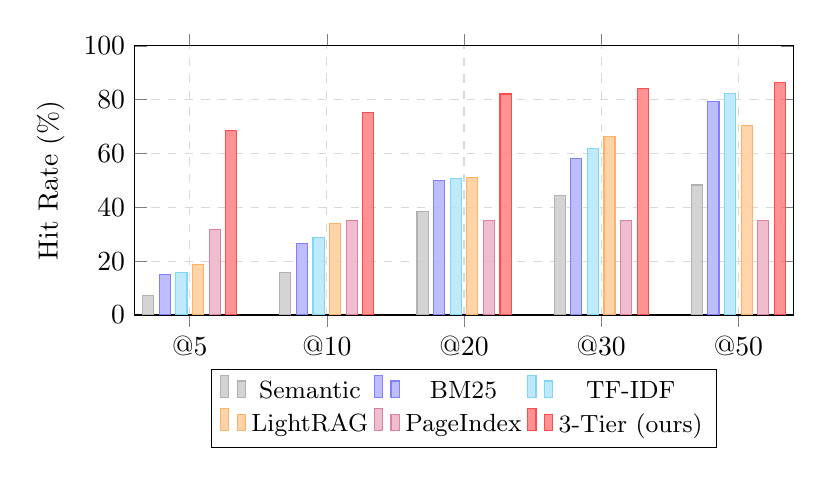
\begin{tikzpicture}
\begin{axis}[
    width=0.82\textwidth,
    height=5cm,
    ybar,
    bar width=4pt,
    ylabel={Hit Rate (\%)},
    symbolic x coords={@5,@10,@20,@30,@50},
    xtick=data,
    ymin=0, ymax=100,
    legend style={at={(0.5,-0.2)}, anchor=north, legend columns=3, font=\small},
    nodes near coords style={font=\tiny, rotate=90, anchor=west},
    every axis plot/.append style={fill opacity=0.85},
    grid=major,
    grid style={dashed, gray!30},
]
\addplot[fill=gray!40, draw=gray!60] coordinates {(@5,7.4) (@10,15.8) (@20,38.5) (@30,44.3) (@50,48.3)};
\addplot[fill=blue!30, draw=blue!50] coordinates {(@5,15.0) (@10,26.7) (@20,50.1) (@30,58.1) (@50,79.2)};
\addplot[fill=cyan!30, draw=cyan!50] coordinates {(@5,15.8) (@10,28.8) (@20,50.7) (@30,62.0) (@50,82.3)};
\addplot[fill=orange!40, draw=orange!60] coordinates {(@5,18.8) (@10,33.9) (@20,51.0) (@30,66.2) (@50,70.3)};
\addplot[fill=purple!30, draw=purple!50] coordinates {(@5,31.7) (@10,35.2) (@20,35.2) (@30,35.2) (@50,35.2)};
\addplot[fill=red!50, draw=red!70] coordinates {(@5,68.5) (@10,75.2) (@20,82.1) (@30,84.0) (@50,86.4)};
\legend{Semantic, BM25, TF-IDF, LightRAG, PageIndex, 3-Tier (ours)}
\end{axis}
\end{tikzpicture}
\caption{Hit@$k$ comparison. Our 3-Tier system consistently outperforms all baselines, with the largest gap at Hit@5 (68.5\% vs.\ 31.7\%).}
\label{fig:hitk-comparison}
\end{figure}

\begin{multicols}{2}

\subsection{Detailed IR Metrics}

Table~\ref{tab:detailed-metrics} reports comprehensive retrieval metrics for our system.

\vspace{0.3em}
\noindent
\centering\small
\captionof{table}{Detailed IR metrics for 3-Tier system.}
\label{tab:detailed-metrics}
\begin{tabular}{lrrrr}
\toprule
\textbf{$k$} & \textbf{Hit@$k$} & \textbf{Recall@$k$} & \textbf{Prec.@$k$} & \textbf{NDCG@$k$} \\
\midrule
1 & 42.7 & 23.9 & 42.7 & 42.7 \\
3 & 62.9 & 41.5 & 26.6 & 41.1 \\
5 & 68.5 & 46.7 & 18.3 & 43.4 \\
10 & 75.2 & 51.8 & 10.3 & 45.4 \\
20 & 82.1 & 59.2 & 6.1 & 47.8 \\
30 & 84.0 & 61.9 & 4.3 & 48.6 \\
50 & 86.4 & 67.4 & 2.9 & 49.9 \\
\bottomrule
\end{tabular}
\normalsize
\justifying
\vspace{0.3em}

MRR is 0.545, indicating the first relevant article appears on average at rank~$\sim$1.8. Recall improves steadily up to $k\!=\!50$, reaching 67.4\%.

\subsection{Ablation Study}

Table~\ref{tab:ablation} isolates each tier's contribution.

\vspace{0.3em}
\noindent
\centering\small
\captionof{table}{Ablation study: per-tier contribution (\%).}
\label{tab:ablation}
\begin{tabular}{lr}
\toprule
\textbf{Configuration} & \textbf{Hit@10} \\
\midrule
Tier 1 only (Tree Traversal) & 56.2 \\
Tier 2 only (DualLevel + PPR) & 61.7 \\
Tier 1 + Tier 2 (no RRF fusion) & 71.2 \\
Full 3-Tier (with Tier 3 RRF) & \textbf{75.2} \\
\bottomrule
\end{tabular}
\normalsize
\justifying
\vspace{0.3em}

Each tier provides additive improvement: Tier~1 alone achieves 56.2\%, adding Tier~2 yields 71.2\% (+15.0pp), and Tier~3 fusion adds 4.0pp to reach 75.2\%. Among successful retrievals, 70\% of hits originate from Tier~1, while Tier~2 contributes 14\% of unique hits not found by Tier~1, confirming complementarity.

\subsection{Analysis}

\subsubsection{Performance by Query Type}

Table~\ref{tab:category-results} breaks down Hit@10 by question category.

\vspace{0.3em}
\noindent
\centering\small
\captionof{table}{Hit@10 by question category (\%).}
\label{tab:category-results}
\begin{tabular}{lrr}
\toprule
\textbf{Category} & \textbf{Hit@10} & \textbf{Count} \\
\midrule
Article lookup & 82.1 & 156 \\
Guidance document & 73.5 & 98 \\
Situation analysis & 71.3 & 75 \\
Compare regulations & 68.8 & 32 \\
Case law lookup & 61.1 & 18 \\
\bottomrule
\end{tabular}
\normalsize
\justifying
\vspace{0.3em}

The system excels on article lookup queries (82.1\%) where Tier~1's structured navigation directly identifies targets. Complex categories like situation analysis and compare regulations benefit from Tier~2's multi-hop reasoning through the knowledge graph.

\subsubsection{Qualitative Analysis}

Figure~\ref{fig:walkthrough} illustrates the three-tier process on a representative query.

\textbf{Success case.} Query: ``Conditions for establishing a joint-stock company?'' Tier~1 navigates Chapter~II $\to$ Articles~111--112, correctly identifying JSC establishment conditions. Tier~2 finds additional Article~17 (general conditions) via \textit{requires} in KG. Tier~3 fuses both, ranking Articles~111, 112, 17 in top~3. Ground truth: Articles~111, 112---\textbf{Hit@3}.

\textbf{Failure case.} Query: ``Penalty for late annual report submission?'' Tier~1 identifies Enterprise Law articles on reporting obligations but misses the penalty, which resides in Decree~122/2021, a separate document. Tier~2's KG expansion partially reaches the decree via \textit{has\_penalty} edges but ranks the penalty article at position~15. This illustrates the challenge of cross-document retrieval when answers span multiple legal instruments.

\subsubsection{Error Analysis}

Analysis of the 93 failed queries (24.8\% of total) reveals three main failure modes: (1)~\textbf{Cross-document gaps} (42\% of failures): the answer resides in a decree not directly linked to the primary law, requiring deeper cross-reference chains. (2)~\textbf{Vietnamese compound term splitting} (28\%): word segmentation errors fragment compound legal terms (e.g., ``tr\'ach nhi\d{e}m h\~{u}u h\d{a}n'' split incorrectly), degrading entity matching. (3)~\textbf{Ambiguous intent} (30\%): queries mixing multiple intents (e.g., ``conditions \textit{and} penalties for...'') cause intent-weighted PPR to prioritize one path over the other.

\end{multicols}

\begin{figure}[H]
\centering
\resizebox{0.92\textwidth}{!}{%
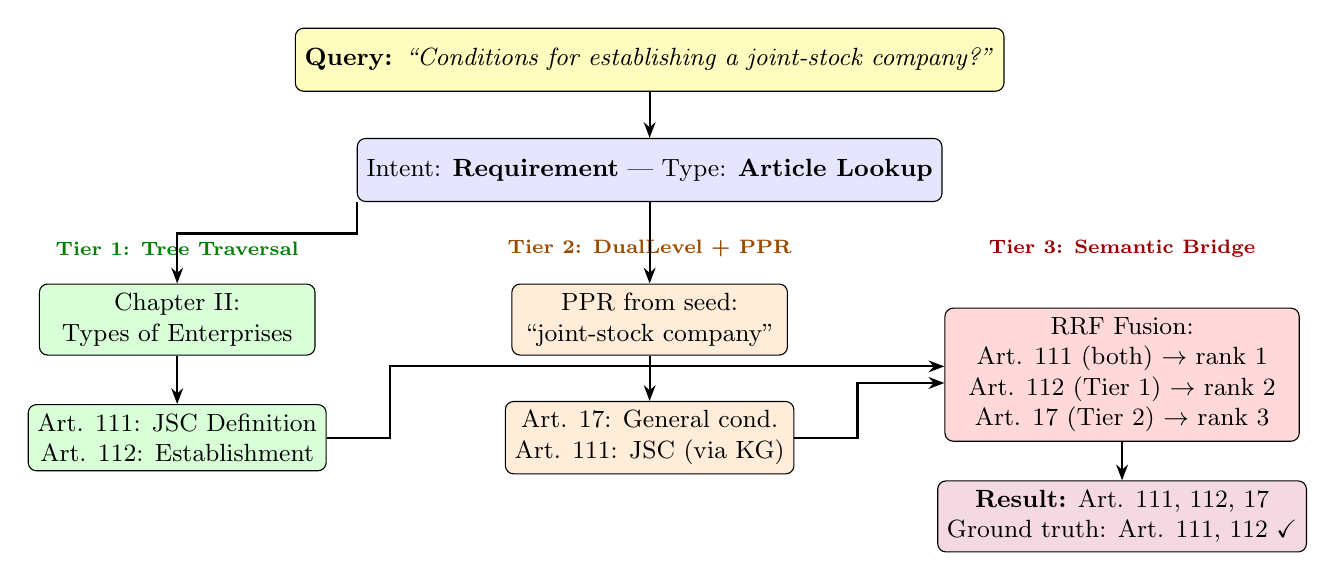
\begin{tikzpicture}[
    box/.style={rectangle, draw, rounded corners=3pt, minimum height=0.8cm, align=center, font=\small},
    arrow/.style={-{Stealth[length=2mm]}, thick},
]
% Query
\node[box, fill=yellow!25, minimum width=7cm] (query) at (0,0) {\textbf{Query:} \textit{``Conditions for establishing a joint-stock company?''}};
\node[box, fill=blue!10, minimum width=5cm] (analyzer) at (0,-1.4) {Intent: \textbf{Requirement} | Type: \textbf{Article Lookup}};
\draw[arrow] (query) -- (analyzer);

% Tier 1
\node[font=\scriptsize\bfseries, green!50!black] at (-6,-2.4) {Tier 1: Tree Traversal};
\node[box, fill=green!15, minimum width=3.5cm] (t1a) at (-6,-3.3) {Chapter II:\\Types of Enterprises};
\node[box, fill=green!15, minimum width=3.5cm] (t1b) at (-6,-4.8) {Art. 111: JSC Definition\\Art. 112: Establishment};
\draw[arrow] (analyzer.south west) -- ++(0,-0.4) -| (t1a.north);
\draw[arrow] (t1a) -- (t1b);

% Tier 2
\node[font=\scriptsize\bfseries, orange!60!black] at (0,-2.4) {Tier 2: DualLevel + PPR};
\node[box, fill=orange!15, minimum width=3.5cm] (t2a) at (0,-3.3) {PPR from seed:\\``joint-stock company''};
\node[box, fill=orange!15, minimum width=3.5cm] (t2b) at (0,-4.8) {Art. 17: General cond.\\Art. 111: JSC (via KG)};
\draw[arrow] (analyzer.south) -- (t2a.north);
\draw[arrow] (t2a) -- (t2b);

% Tier 3
\node[font=\scriptsize\bfseries, red!60!black] at (6,-2.4) {Tier 3: Semantic Bridge};
\node[box, fill=red!15, minimum width=4.5cm] (t3) at (6,-4.0) {RRF Fusion:\\Art. 111 (both) $\rightarrow$ rank 1\\Art. 112 (Tier 1) $\rightarrow$ rank 2\\Art. 17 (Tier 2) $\rightarrow$ rank 3};
\draw[arrow] (t1b.east) -- ++(0.8,0) |- ([yshift=3pt]t3.west);
\draw[arrow] (t2b.east) -- ++(0.8,0) |- ([yshift=-3pt]t3.west);

% Result
\node[box, fill=purple!15, minimum width=4.5cm] (result) at (6,-5.8) {\textbf{Result:} Art. 111, 112, 17\\Ground truth: Art. 111, 112 $\checkmark$};
\draw[arrow] (t3) -- (result);
\end{tikzpicture}
}
\caption{Query walkthrough. Tier~1 navigates the document tree, Tier~2 uses PPR on the knowledge graph, and Tier~3 fuses results via RRF.}
\label{fig:walkthrough}
\end{figure}

\begin{multicols}{2}

\textbf{Reproducibility.} All LLM responses are cached in SQLite ($\sim$1.1\,GB), making results fully deterministic. Standard deviations are zero and not reported.

\section{Discussion}
\label{sec:discussion}

Three findings emerge from our experiments. First, the tiers are \textbf{complementary rather than redundant}: Tier~1 excels at focused article identification via structural reasoning (70\% of hits), while Tier~2 captures cross-reference and thematic relationships (14\% unique hits). The 15pp gain from adding Tier~2 to Tier~1 confirms that structural and semantic retrieval address different failure modes.

Second, \textbf{intent-aware PPR} is particularly effective for situation analysis and guidance queries, where traversing the correct relation types (e.g., \textit{requires} for procedures, \textit{has\_authority} for rights) substantially improves ranking. The weight matrix (Table~\ref{tab:intent-weights}) encodes legal domain knowledge that general-purpose graph traversal lacks.

Third, \textbf{document structure matters more than flat search}: PageIndex (35.2\% Hit@10 with 3.9 articles) matches LightRAG (33.9\% with 32.8 articles), retrieving equivalent accuracy with an order of magnitude fewer articles. This validates the value of hierarchical navigation in legal corpora.

The knowledge representation model $\mathcal{M}$ provides a principled framework for organizing legal knowledge across complementary representations. By separating terminological ($\mathcal{O}$), assertional ($\mathcal{G}$), and structural ($\mathcal{T}$) knowledge, each retrieval tier can specialize in its strength while the fusion tier integrates their contributions.

\section{Conclusion}
\label{sec:conclusion}

We presented a three-tier knowledge graph RAG system for Vietnamese legal QA that extends the Legal-Onto Rela-model with a formal knowledge model $\mathcal{M} = (\mathcal{O}, \mathcal{G}, \mathcal{T}, \Phi)$. The system combines LLM-guided structural navigation, dual-level semantic retrieval with intent-aware Personalized PageRank, and Reciprocal Rank Fusion. Experiments on 375 real questions demonstrate 75.2\% Hit@10 (MRR 0.545), outperforming baselines by 41.3 percentage points. Ablation studies confirm each tier's additive contribution.

\textbf{Limitations.} Tree traversal requires multiple LLM calls per query ($\sim$7s latency). Entity extraction accuracy for Vietnamese legal text has not been independently validated. Results are specific to Enterprise Law; other legal domains may exhibit different retrieval patterns.

\textbf{Future work.} We plan to: (1)~extend the knowledge graph to cover related laws (Investment, Tax, Labor) with cross-law entity resolution, (2)~add multi-turn conversation support for follow-up questions, (3)~develop advanced 3+ hop KG reasoning for complex transitive inference, and (4)~build explainable retrieval traces showing tier and ontology path contributions.

\section*{Acknowledgments}

This research was supported by Vietnam National University Ho Chi Minh City under grant number [Grant Number]. We thank the legal experts who contributed to ontology validation and ground truth annotation.

\end{multicols}

\begin{thebibliography}{99}
\footnotesize
\setlength{\itemsep}{0pt}
\setlength{\parskip}{0pt}

\bibitem{ref1}
Robertson, S., Zaragoza, H.: The Probabilistic Relevance Framework: BM25 and Beyond. Foundations and Trends in Information Retrieval \textbf{3}(4), 333--389 (2009)

\bibitem{ref2}
Lewis, P., Perez, E., Piktus, A., et al.: Retrieval-Augmented Generation for Knowledge-Intensive NLP Tasks. In: NeurIPS 2020, pp. 9459--9474 (2020)

\bibitem{ref3}
Karpukhin, V., Oguz, B., Min, S., et al.: Dense Passage Retrieval for Open-Domain Question Answering. In: EMNLP 2020, pp. 6769--6781 (2020)

\bibitem{ref4}
Microsoft Research: From Local to Global: A Graph RAG Approach to Query-Focused Summarization. arXiv preprint arXiv:2404.16130 (2024)

\bibitem{ref5}
Guo, Z., et al.: LightRAG: Simple and Fast Retrieval-Augmented Generation. arXiv preprint arXiv:2410.05779 (2024)

\bibitem{ref6}
Nguyen, T., Nguyen, H., Pham, V., Tran, D., Selamat, A.: Legal-Onto: An Ontology-based Model for Representing the Knowledge of a Legal Document. In: ENASE 2022, pp. 426--434 (2022)

\bibitem{ref7}
Ngo, H., Nguyen, T., Nguyen, D., Pham, M.: AimeLaw at ALQAC 2021: Enriching Neural Network Models with Legal-Domain Knowledge. In: KSE 2021. IEEE (2021)

\bibitem{ref8}
Sartor, G., et al.: Approaches to Legal Ontologies. Springer, Dordrecht (2011)

\bibitem{ref9}
Es, S., James, J., Espinosa-Anke, L., Schockaert, S.: RAGAS: Automated Evaluation of Retrieval Augmented Generation. In: EACL 2024 (2024)

\bibitem{ref10}
Do, N., Nguyen, H., Selamat, A.: Knowledge-Based model of Expert Systems using Rela-model. International Journal of Software Engineering and Knowledge Engineering \textbf{28}(8), 1047--1090 (2018)

\bibitem{ref11}
Manning, C., Raghavan, P., Schutze, H.: Introduction to Information Retrieval. Cambridge University Press (2008)

\bibitem{ref12}
Gleich, D.: PageRank Beyond the Web. SIAM Review \textbf{57}(3), 321--363 (2015)

\bibitem{ref13}
Devlin, J., Chang, M., Lee, K., Toutanova, K.: BERT: Pre-training of Deep Bidirectional Transformers for Language Understanding. In: NAACL-HLT 2019, pp. 4171--4186 (2019)

\bibitem{ref14}
Liu, Z., et al.: Retrieve Anything To Augment Large Language Models. arXiv preprint arXiv:2310.07554 (2023)

\bibitem{ref_gao2024}
Gao, Y., Xiong, Y., Diber, A., et al.: Retrieval-Augmented Generation for Large Language Models: A Survey. arXiv preprint arXiv:2312.10997 (2024)

\bibitem{ref_fan2024}
Fan, W., Ding, Y., Ning, L., et al.: A Survey on RAG Meeting LLMs: Towards Retrieval-Augmented Large Language Models. In: KDD 2024, pp. 6491--6501 (2024)

\bibitem{ref_phobert}
Nguyen, D.Q., Nguyen, A.T.: PhoBERT: Pre-trained Language Models for Vietnamese. In: Findings of EMNLP 2020, pp. 1037--1042 (2020)

\bibitem{ref_vncorenlp}
Vu, T., Nguyen, D.Q., Nguyen, D.Q., Dras, M., Johnson, M.: VnCoreNLP: A Vietnamese Natural Language Processing Toolkit. In: NAACL 2018 Demonstrations, pp. 56--60 (2018)

\bibitem{ref_transe}
Bordes, A., Usunier, N., Garcia-Duran, A., Weston, J., Yakhnenko, O.: Translating Embeddings for Modeling Multi-relational Data. In: NeurIPS 2013, pp. 2787--2795 (2013)

\bibitem{ref_jeh2003}
Jeh, G., Widom, J.: Scaling Personalized Web Search. In: WWW 2003, pp. 271--279. ACM (2003)

\bibitem{ref_rrf}
Cormack, G.V., Clarke, C.L.A., Buettcher, S.: Reciprocal Rank Fusion Outperforms Condorcet and Individual Rank Learning Methods. In: SIGIR 2009, pp. 758--759. ACM (2009)

\bibitem{ref_sbert}
Reimers, N., Gurevych, I.: Sentence-BERT: Sentence Embeddings using Siamese BERT-Networks. In: EMNLP 2019, pp. 3982--3992 (2019)

\bibitem{ref_selfrag}
Asai, A., Wu, Z., Wang, Y., Sil, A., Hajishirzi, H.: Self-RAG: Learning to Retrieve, Generate, and Critique through Self-Reflection. In: ICLR 2024 (2024)

\bibitem{ref_crag}
Yan, S.Q., et al.: Corrective Retrieval Augmented Generation. arXiv preprint arXiv:2401.15884 (2024)

\bibitem{ref_hyde}
Gao, L., Ma, X., Lin, J., Callan, J.: Precise Zero-Shot Dense Retrieval without Relevance Labels. In: ACL 2023, pp. 1762--1777 (2023)

\bibitem{ref_wadhwa}
Wadhwa, S., Amir, S., Wallace, B.C.: Revisiting Relation Extraction in the Era of Large Language Models. In: ACL 2023, pp. 15566--15589 (2023)

\bibitem{ref_chalkidis}
Chalkidis, I., Fergadiotis, M., Malakasiotis, P., Aletras, N., Androutsopoulos, I.: LEGAL-BERT: The Muppets Straight out of Law School. In: Findings of EMNLP 2020, pp. 2898--2904 (2020)

\bibitem{ref_zhong2020}
Zhong, H., Xiao, C., Tu, C., Zhang, T., Liu, Z., Sun, M.: How Does NLP Benefit Legal System: A Summary of Legal Artificial Intelligence. In: ACL 2020, pp. 5218--5230 (2020)

\bibitem{ref_vaswani}
Vaswani, A., Shazeer, N., Parmar, N., et al.: Attention Is All You Need. In: NeurIPS 2017, pp. 5998--6008 (2017)

\bibitem{ref_rotateE}
Sun, Z., Deng, Z.-H., Nie, J.-Y., Tang, J.: RotatE: Knowledge Graph Embedding by Relational Rotation in Complex Space. In: ICLR 2019 (2019)

\bibitem{ref_legalai2024}
Cui, J., Li, X., Shao, Z., et al.: A Survey on Legal Large Language Models. arXiv preprint arXiv:2312.03718 (2024)

\end{thebibliography}

\vspace{0.5em}
\hrule
\vspace{0.3em}
\footnotesize
$^1$Corresponding Author: Le Hong Hien, Faculty of Computer Science, University of Information Technology, Vietnam National University Ho Chi Minh City, Vietnam; E-mail: hienlh.16@grad.uit.edu.vn.

\end{document}
